\documentclass[11pt]{article}
\usepackage[utf8]{inputenc}
\usepackage[english]{babel}
\usepackage{bilal2vec}

\title{SE 380 — P1}
\author{Bilal Khan\\
\href{mailto:b54khan@uwaterloo.ca}{b54khan@uwaterloo.ca}\\
Bohdan Hrotovytskyy\\
\href{mailto:bhrotovy@uwaterloo.ca}{bhrotovy@uwaterloo.ca}}
\date{\today}

\begin{document}

\maketitle

\tableofcontents

\section{Task 1}

To run the code properly and plot all the figures copy the code into a jupyter notebook and run each plot cell individually.

\subsection{Item 1}

Our inputs $u = [u_1, u_2]^T$ are constant values of $1$ over a time period of $15$ seconds where one timestep lasts $0.001$s. In numpy, we can represent this as a two-dimensional vector of length $15,000$: \mintinline{python}{u = np.ones((15,000, 2))}.

We can generate the two output signals $y = [y_1, y_2]^2$ by passing the inputs through the simulator \mintinline{python}{y = sm.sim(u)}

\subsection{Item 2}

We plot the two input signals and two output signals below:

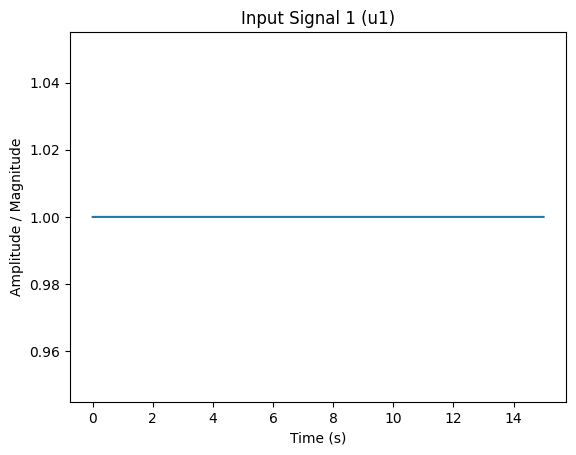
\includegraphics[width=200pt]{p1_1.png}
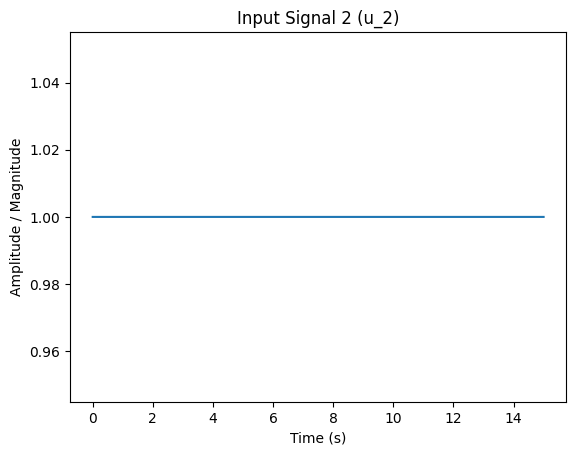
\includegraphics[width=200pt]{p1_2.png}

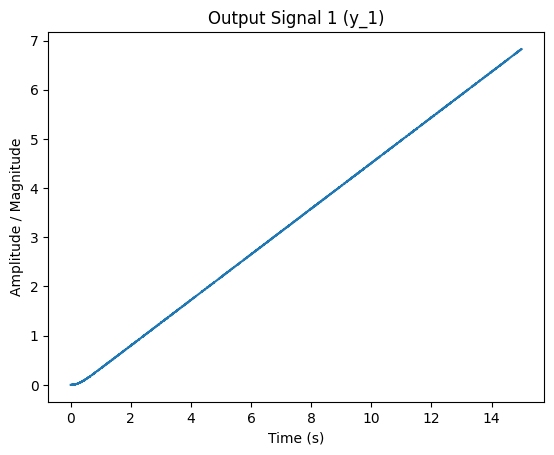
\includegraphics[width=200pt]{p1_3.png}
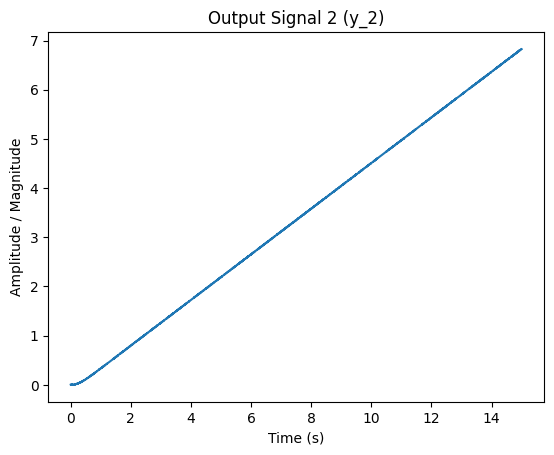
\includegraphics[width=200pt]{p1_4.png}

\subsection{Item 3}

To plot the frequency spectrum of the output signals we use \mintinline{python}{np.fft.fft()} to compute the discrete Fast Fourier Transform on the output signals. Note that we do not plot the negative frequencies (the second half of the output of \mintinline{python}{np.fft.fft()}) and that we can plot the magnitude of the complex numbers returned by \mintinline{python}{np.fft.fft()} using \mintinline{python}{np.abs()}.

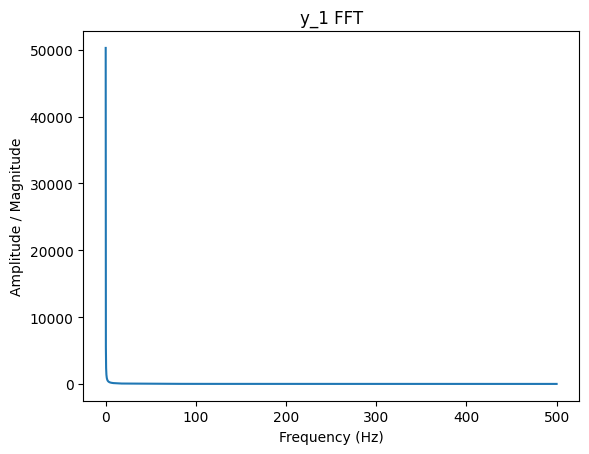
\includegraphics[width=200pt]{p1_5.png}
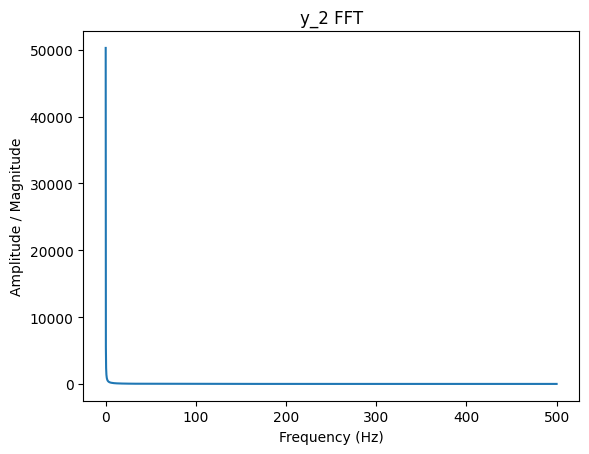
\includegraphics[width=200pt]{p1_6.png}

\subsection{Item 4}

We're going to choose a frequency cutoff to filter out any frequencies larger that $\omega_c$. To do this, note that most of the total energy of the signal is concentrated in frequencies close to zero with a long tail of high frequency components that don't significantly contribute to the signal. Lets plot the same graph but with the frequencies on a log scale (note that this is using \mintinline{python}{np.log}, which uses base $e$): 

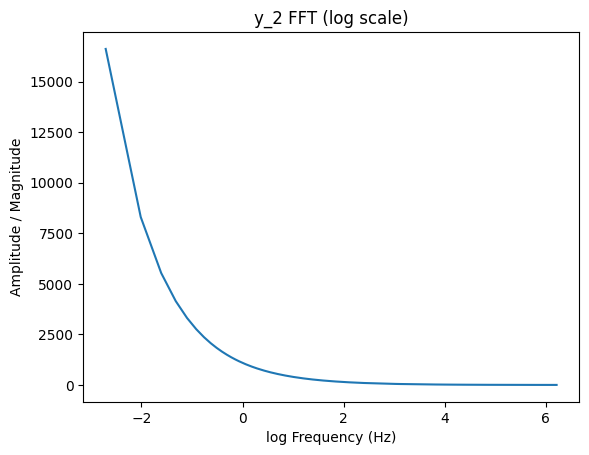
\includegraphics[width=200pt]{p1_7.png}

Looking at this graph, we can see that some reasonable values for $\omega_c$ could be somewhere around the $e^0$ to $e^2$ range since the overwhelming majority of the energy of the signal is already below zero log-frequency. We'll choose $\omega_c = e^1$ as a middle ground for our low pass filter.

\subsection{Item 5}

We'll follow the approach in class and design a low-pass filter as a transfer function in the Laplace/Fourier domain of the format $\dfrac{1}{(s \tau + 1)^3}$, where $\tau = \dfrac{1}{\omega_c}$ is our time constant and $s$ is the Laplace input variable. Since the question asks us to design a third-order filter with multiple real poles that are coincident, we can see that our transfer function has three real poles, all at the same spot due to the cubed term.

\subsection{Item 6}

Since our chosen $\omega_c$ frequency taken from inspecting the graph is in Hertz we will convert it to radians/s and then take the reciprocal to get $\tau$: $\tau = \dfrac{1}{2\pi \omega_c} = \dfrac{1}{2\pi}$. We can then apply the filter by computing the output signals to the Laplace/Fourier domain, multiply them by the transfer function, then convert back to the time domain using the Inverse Fast Fourier Transform. We can do this using the \mintinline{python}{np.fft.ifft()} function.

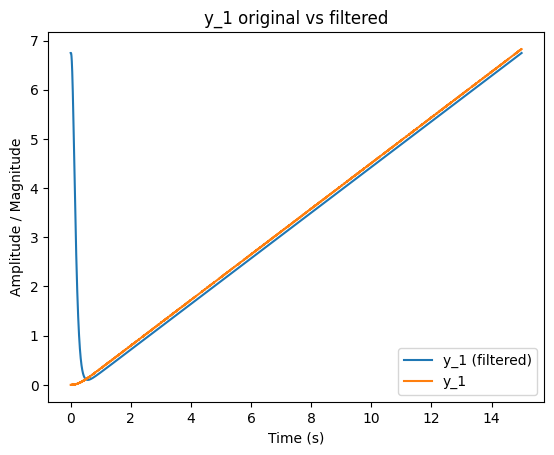
\includegraphics[width=200pt]{p1_8.png}

Looking at the original vs filtered signals, we can see that the filtered signal is a good approximation of the original signal, but with some differences near the beginning due to the lack of high-frequency components.

\end{document}
